\documentclass[paper=a4, fontsize=11pt]{scrartcl} % A4 paper and 11pt font size
\usepackage{graphicx}
\usepackage[polish]{babel}
\usepackage[OT4]{fontenc} 
\usepackage[utf8]{inputenc}
\usepackage[T1]{fontenc} % Use 8-bit encoding that has 256 glyphs
\usepackage{fourier} % Use the Adobe Utopia font for the document - comment this line to return to the LaTeX default
\usepackage[polish]{babel} % English language/hyphenation
\usepackage{amsmath,amsfonts,amsthm} % Math packages
\usepackage{listings}
\usepackage{geometry}
\geometry{bottom=20pt}
\usepackage{sectsty} % Allows customizing section commands
\allsectionsfont{\centering \normalfont\scshape} % Make all sections centered, the default font and small caps

\usepackage{fancyhdr} % Custom headers and footers
\pagestyle{fancyplain} % Makes all pages in the document conform to the custom headers and footers
\fancyhead{} % No page header - if you want one, create it in the same way as the footers below
\fancyfoot[L]{} % Empty left footer
\fancyfoot[C]{} % Empty center footer
\fancyfoot[R]{\thepage} % Page numbering for right footer
\renewcommand{\headrulewidth}{0pt} % Remove header underlines
\renewcommand{\footrulewidth}{0pt} % Remove footer underlines
\setlength{\headheight}{-70pt} % Customize the height of the header

\numberwithin{equation}{section} % Number equations within sections (i.e. 1.1, 1.2, 2.1, 2.2 instead of 1, 2, 3, 4)
\numberwithin{figure}{section} % Number figures within sections (i.e. 1.1, 1.2, 2.1, 2.2 instead of 1, 2, 3, 4)
\numberwithin{table}{section} % Number tables within sections (i.e. 1.1, 1.2, 2.1, 2.2 instead of 1, 2, 3, 4)


\usepackage{color}

\definecolor{mygreen}{rgb}{0,0.6,0}
\definecolor{mygray}{rgb}{0.5,0.5,0.5}
\definecolor{mymauve}{rgb}{0.58,0,0.82}

\lstset{ %
	backgroundcolor=\color{white},   % choose the background color; you must add \usepackage{color} or \usepackage{xcolor}
	basicstyle=\footnotesize,        % the size of the fonts that are used for the code
	breakatwhitespace=false,         % sets if automatic breaks should only happen at whitespace
	breaklines=true,                 % sets automatic line breaking
	captionpos=b,                    % sets the caption-position to bottom
	commentstyle=\color{mygreen},    % comment style
	deletekeywords={...},            % if you want to delete keywords from the given language
	escapeinside={\%*}{*)},          % if you want to add LaTeX within your code
	extendedchars=true,              % lets you use non-ASCII characters; for 8-bits encodings only, does not work with UTF-8
	frame=single,                    % adds a frame around the code
	keepspaces=true,                 % keeps spaces in text, useful for keeping indentation of code (possibly needs columns=flexible)
	keywordstyle=\color{blue},       % keyword style
	language=Octave,                 % the language of the code
	morekeywords={*,...},            % if you want to add more keywords to the set
	numbers=left,                    % where to put the line-numbers; possible values are (none, left, right)
	numbersep=5pt,                   % how far the line-numbers are from the code
	numberstyle=\tiny\color{mygray}, % the style that is used for the line-numbers
	rulecolor=\color{black},         % if not set, the frame-color may be changed on line-breaks within not-black text (e.g. comments (green here))
	showspaces=false,                % show spaces everywhere adding particular underscores; it overrides 'showstringspaces'
	showstringspaces=false,          % underline spaces within strings only
	showtabs=false,                  % show tabs within strings adding particular underscores
	stepnumber=2,                    % the step between two line-numbers. If it's 1, each line will be numbered
	stringstyle=\color{mymauve},     % string literal style
	tabsize=2,                       % sets default tabsize to 2 spaces
	title=\lstname                   % show the filename of files included with \lstinputlisting; also try caption instead of title
}
\setlength\parindent{0pt} % Removes all indentation from paragraphs - comment this line for an assignment with lots of text

%----------------------------------------------------------------------------------------
%	TITLE SECTION
%----------------------------------------------------------------------------------------

\newcommand{\horrule}[1]{\rule{\linewidth}{#1}} % Create horizontal rule command with 1 argument of height

\title{	
\normalfont \normalsize 
\textsc{Wydział Fizyki i Astronomii\\Uniwersytet Wrocławski} \\ [25pt] % Your university, school and/or department name(s)
\horrule{0.5pt} \\[0.4cm] % Thin top horizontal rule
\huge Projekt CUDA \\ % The assignment title
\horrule{2pt} \\[0.5cm] % Thick bottom horizontal rule
}

\author{Paweł Grabiński} % Your name

\date{\normalsize\today} % Today's date or a custom date

\begin{document}

\maketitle % Print the title

%----------------------------------------------------------------------------------------
%	PROBLEM 1
%----------------------------------------------------------------------------------------

\section{Obliczenia równoległe przy użyciu technologii Nvidia Cuda}


\subsection{Treść problemu}
\center\large{Wybrane zadanie: nr $9$}\\
\normalsize Napisz program, który na GPU rozwiąże następujący problem: dany jest ciąg trójek liczb $ \left( x_i, y_i, z_i\right) , i = 0,...,N-1$, definiujących współrzędne środków gwiazd w przestrzeni oraz $N$-elementowa tablica $v$ przekazana poprzez wskaźnik do pierwszego elementu. W środku układu współrzędnych znajduje się Bardo Masywny Obiekt i interesują nas energie potencjalne gwiazd w polu grawitacyjnym Obiektu. 
\begin{itemize}
\item	Napisz program, który w elemencie $i$ tablicy $v$, $ i = 0,...,N-1$, zapisze odwrotność odległości punktu $ \left( x_i, y_i, z_i\right)$ od środka układu współrzędnych.  
\item Przetestuj efektywność swojego programu dla kilku wartości $N$.
\item Porównaj wydajność swojego rozwiązania z wydajnością analogicznego programu rozwiązującego ten problem na CPU.  
\end{itemize}
Uwaga: Trójki liczb zmiennopozycyjnych wygodnie zapisuje się w typie float3 lub double3. Możesz też użyć typów float4 i double4 i założyć, że potencjały zapisuje się w czwartej składowej tych struktur zamiast w tablicy $v$. 

\subsection{Metodologia rozwiązania}
Podczas pracy programu zachodzą następujące działania:
\begin{enumerate}
\item Na wejściu obliczeń podana musi zostać liczba obiektów $N$ oraz rozmiar obszaru w jakim mogą się znajdować $Size$.
\item Dalej generowane są współrzędne danych obiektów. Liczby generowane są przy pomocy algorytmu Mersenne Twister zaimplementowanego w blibliotece GSL.
\item Zapis danych odbywa się w zmiennych typu float4, co ma zoptymalizować proces przesyłu danych do i z karty graficznej. W trzech pierwszych składowych tej zmiennej zapisujemy współrzędne obiektu, a w czwartej wartość odwrotności odległości.
\item Następnie dane przesyłane są na kartę.
\item Inicjalizowany jest kernel na GPU, który dla każdego elementu wywołuje wątek obliczający odwrotność odległości tego punktu od środka układu i zapisuje go w czwartej składowej przesłanej tablicy.
\item Dane są przesyłane z powrotem z karty.
\item Po tym na CPU uruchamiana jest analogiczna funkcja, która szeregowo oblicza odwrotności odległości punktów.
\end{enumerate}
Czas pracy funkcji obliczeniowych mierzony jest przy pomocy funkcji $clock\_gettime(CLOCK\_MONOTONIC,\&timer)$ z dokładnością do $1\: ns$.
\subsection{Wyniki}
By zbadać jak wydajnym rozwiązaniem jest obliczanie na GPU w porównianiu do CPU zbadaliśmy zależność czasu wykonywania funkcji od ilości elementów układu.
\begin{figure}[h]
\centering
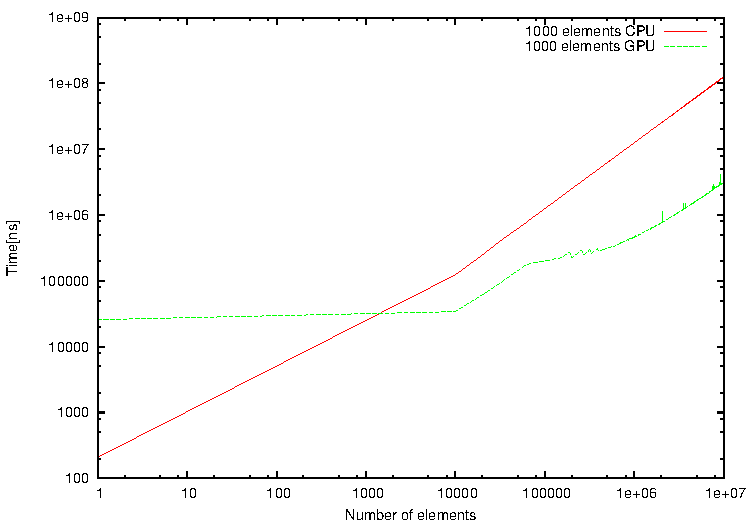
\includegraphics[width=0.6\textwidth]{timesa.pdf}
\label{.}
\end{figure}\\
Wykres ma logarytmiczne osie. Widzimy, że czas wykonania zależy od ilości elementów. Początkowo czas CPU jest znacznie mniejszy od czasu wykonania na GPU, jednak wraz ze wzrostem liczby elementów rośnie on zancznie szybciej niż na GPU. \\ 
Jak widzimy początkowo koszt inicjalizacji kernela jest znacznie większy od czasu wykonania samych obliczeń.\\
Istotną uwagą jest fakt, że porównywanie szeregowych obliczeń do równoległych jest nierozsądne. Adekwatnym byłoby porównywanie równoległych obliczeń na CPU do równoległych na GPU.\\
Isotnym czynnikiem jest także odpowiednia manipulacja wczytywaniem danych. W funkcji $PotentialOnDevice()$ wprowadzenie jednokrotnego wczytywania elementu tablicy typu $float4$ przy $4\times 10^7$ elementów zmieniło czas wykonania z $22\:ms$ do $16\:ms$, co jest istotnym wzrostem efektywności.
\newpage
\subsection{Kod źródłowy rozwiązania}
\lstinputlisting[language=C]{Galaxy.c}
\end{document}